% 第五章 异质性分析:连续剂量(p50)
\paragraph{连续剂量异质性:政策前对处理行业的暴露度(p50)}
\label{sec:chap5_network_heterogeneity}

为提升统计功效并避免阈值选择带来的不稳定性,本节采用\emph{连续剂量}方式刻画政策前“对处理行业的暴露度”\(Z^{pre}_{ij}\),并在事件研究中加入交互项进行估计:
\(II_{ijt} \sim \sum_k\big[\beta_k\,\mathbb{1}\{t=k\}\times Affected_i\big] + \sum_k\big[\gamma_k\,\mathbb{1}\{t=k\}\times Affected_i\times Z^{pre}_{ij,\,std}\big] + X_{ijt}+\mu_{ij}+\lambda_t\)。其中 \(Z^{pre}_{ij,\,std}\) 为标准化剂量。基于交互后的边际效应,我们在\textbf{中位暴露(p50)}处读取“处理×事件”的动态系数并报告(低/高分位曲线见附录)。交互项和代表值的解释遵循 \citet{brambor2006understanding} 与边际效应文献(如 \citet{williams2012margins})。

\paragraph{口径与设定}
与主回归严格一致:样本期 2010–2018;政策时点 2014-01(基准年 -1=2013);因变量 \(II\) 5\% 双侧缩尾;控制变量为 \(i/j\) 两侧的杠杆、ROA、\(\log\)TobinQ;固定效应为配对(pair)与年份(year);标准误在配对层聚类。暴露口径报告三类:\textbf{out}(向处理行业的输出暴露)、\textbf{in}(来自处理行业的输入暴露)与 \textbf{total}(out+in 的综合暴露),配对聚合使用 \(\max\)。

\paragraph{主要结果(p50)}
- 平行趋势:在 \textbf{p50} 处,\textbf{out} 与 \textbf{total} 两种暴露口径的政策前事件系数(k=−4,−3,−2)均不显著(p>0.05),通过平行趋势检验。
- 政策后:\textbf{out} 在 k=1(以及若干后续期)边际效应显著为负;\textbf{total} 在 k=1 显著为负。交互项(处理×事件×\(Z\))在政策后整体为负,并呈现剂量—响应关系(联合检验见附录)。

\begin{figure}[!htbp]
  \centering
  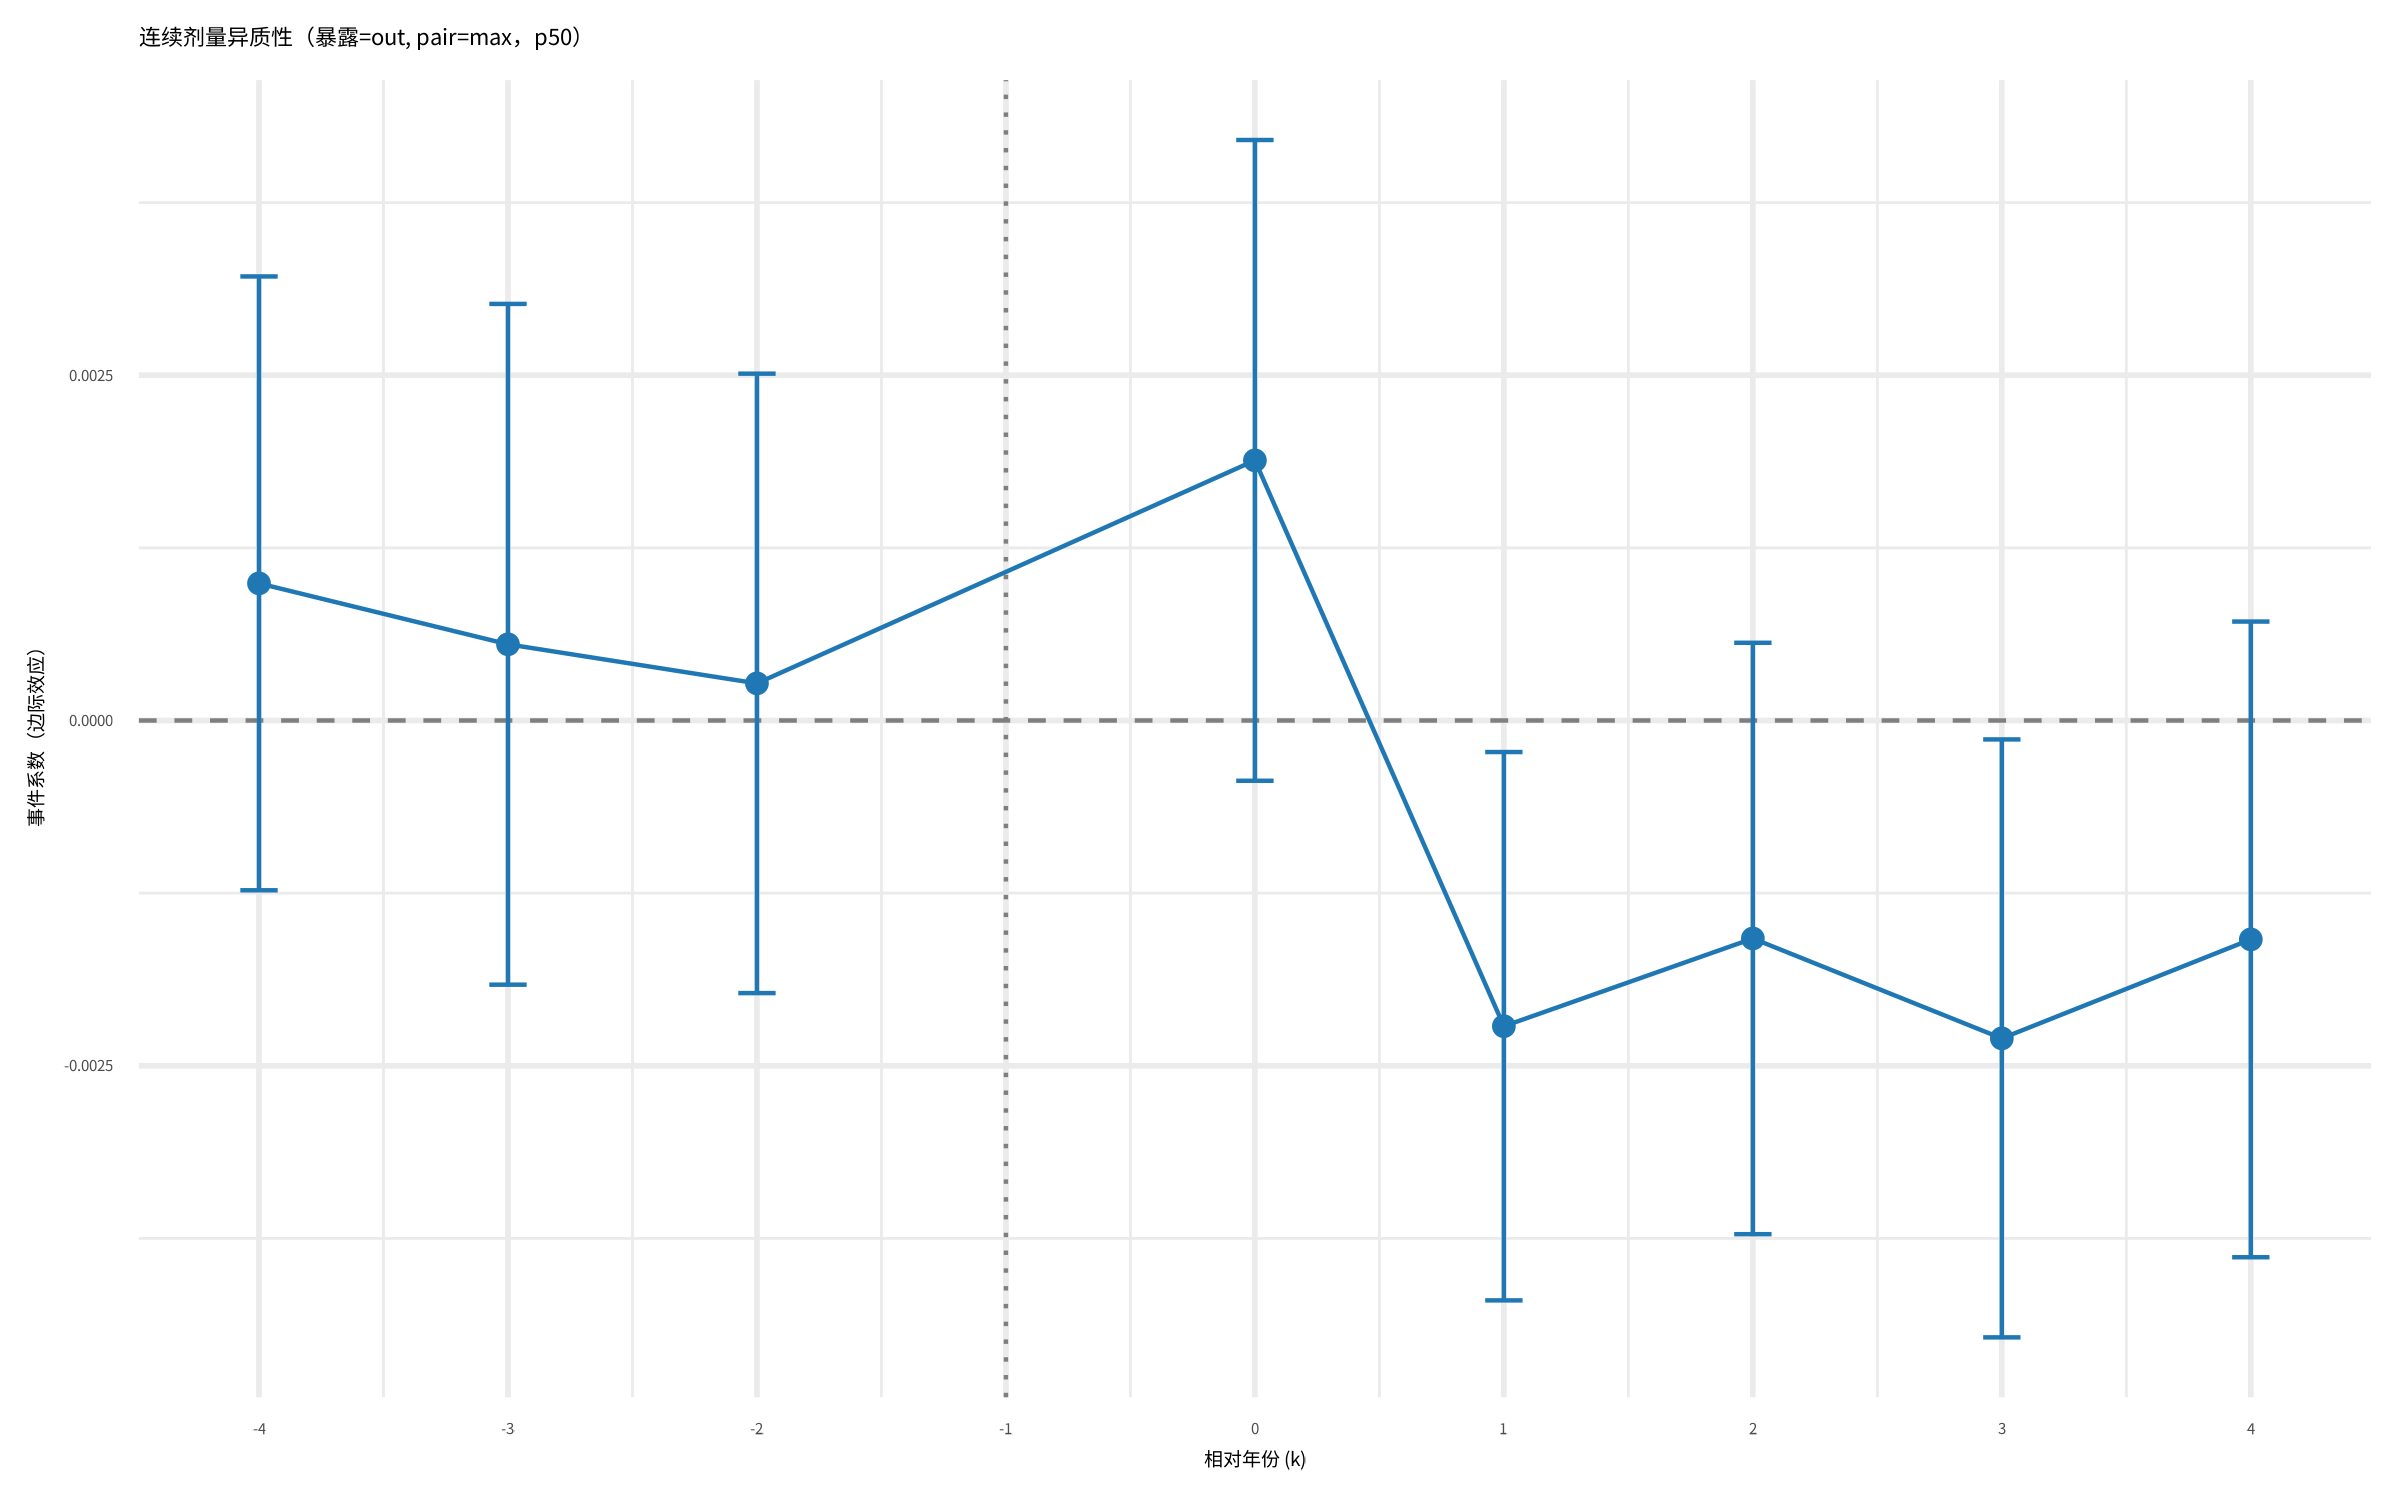
\includegraphics[width=0.85\linewidth]{figures/PT_exposure_cont_out_max_cont_p50.png}
  \caption{连续剂量(\(out\), pair=\(\max\)):中位暴露(p50)事件研究系数(95\%CI)。基准年 -1=2013。}
  \label{fig:hetero_expo_cont_out_p50}
\end{figure}

\begin{figure}[!htbp]
  \centering
  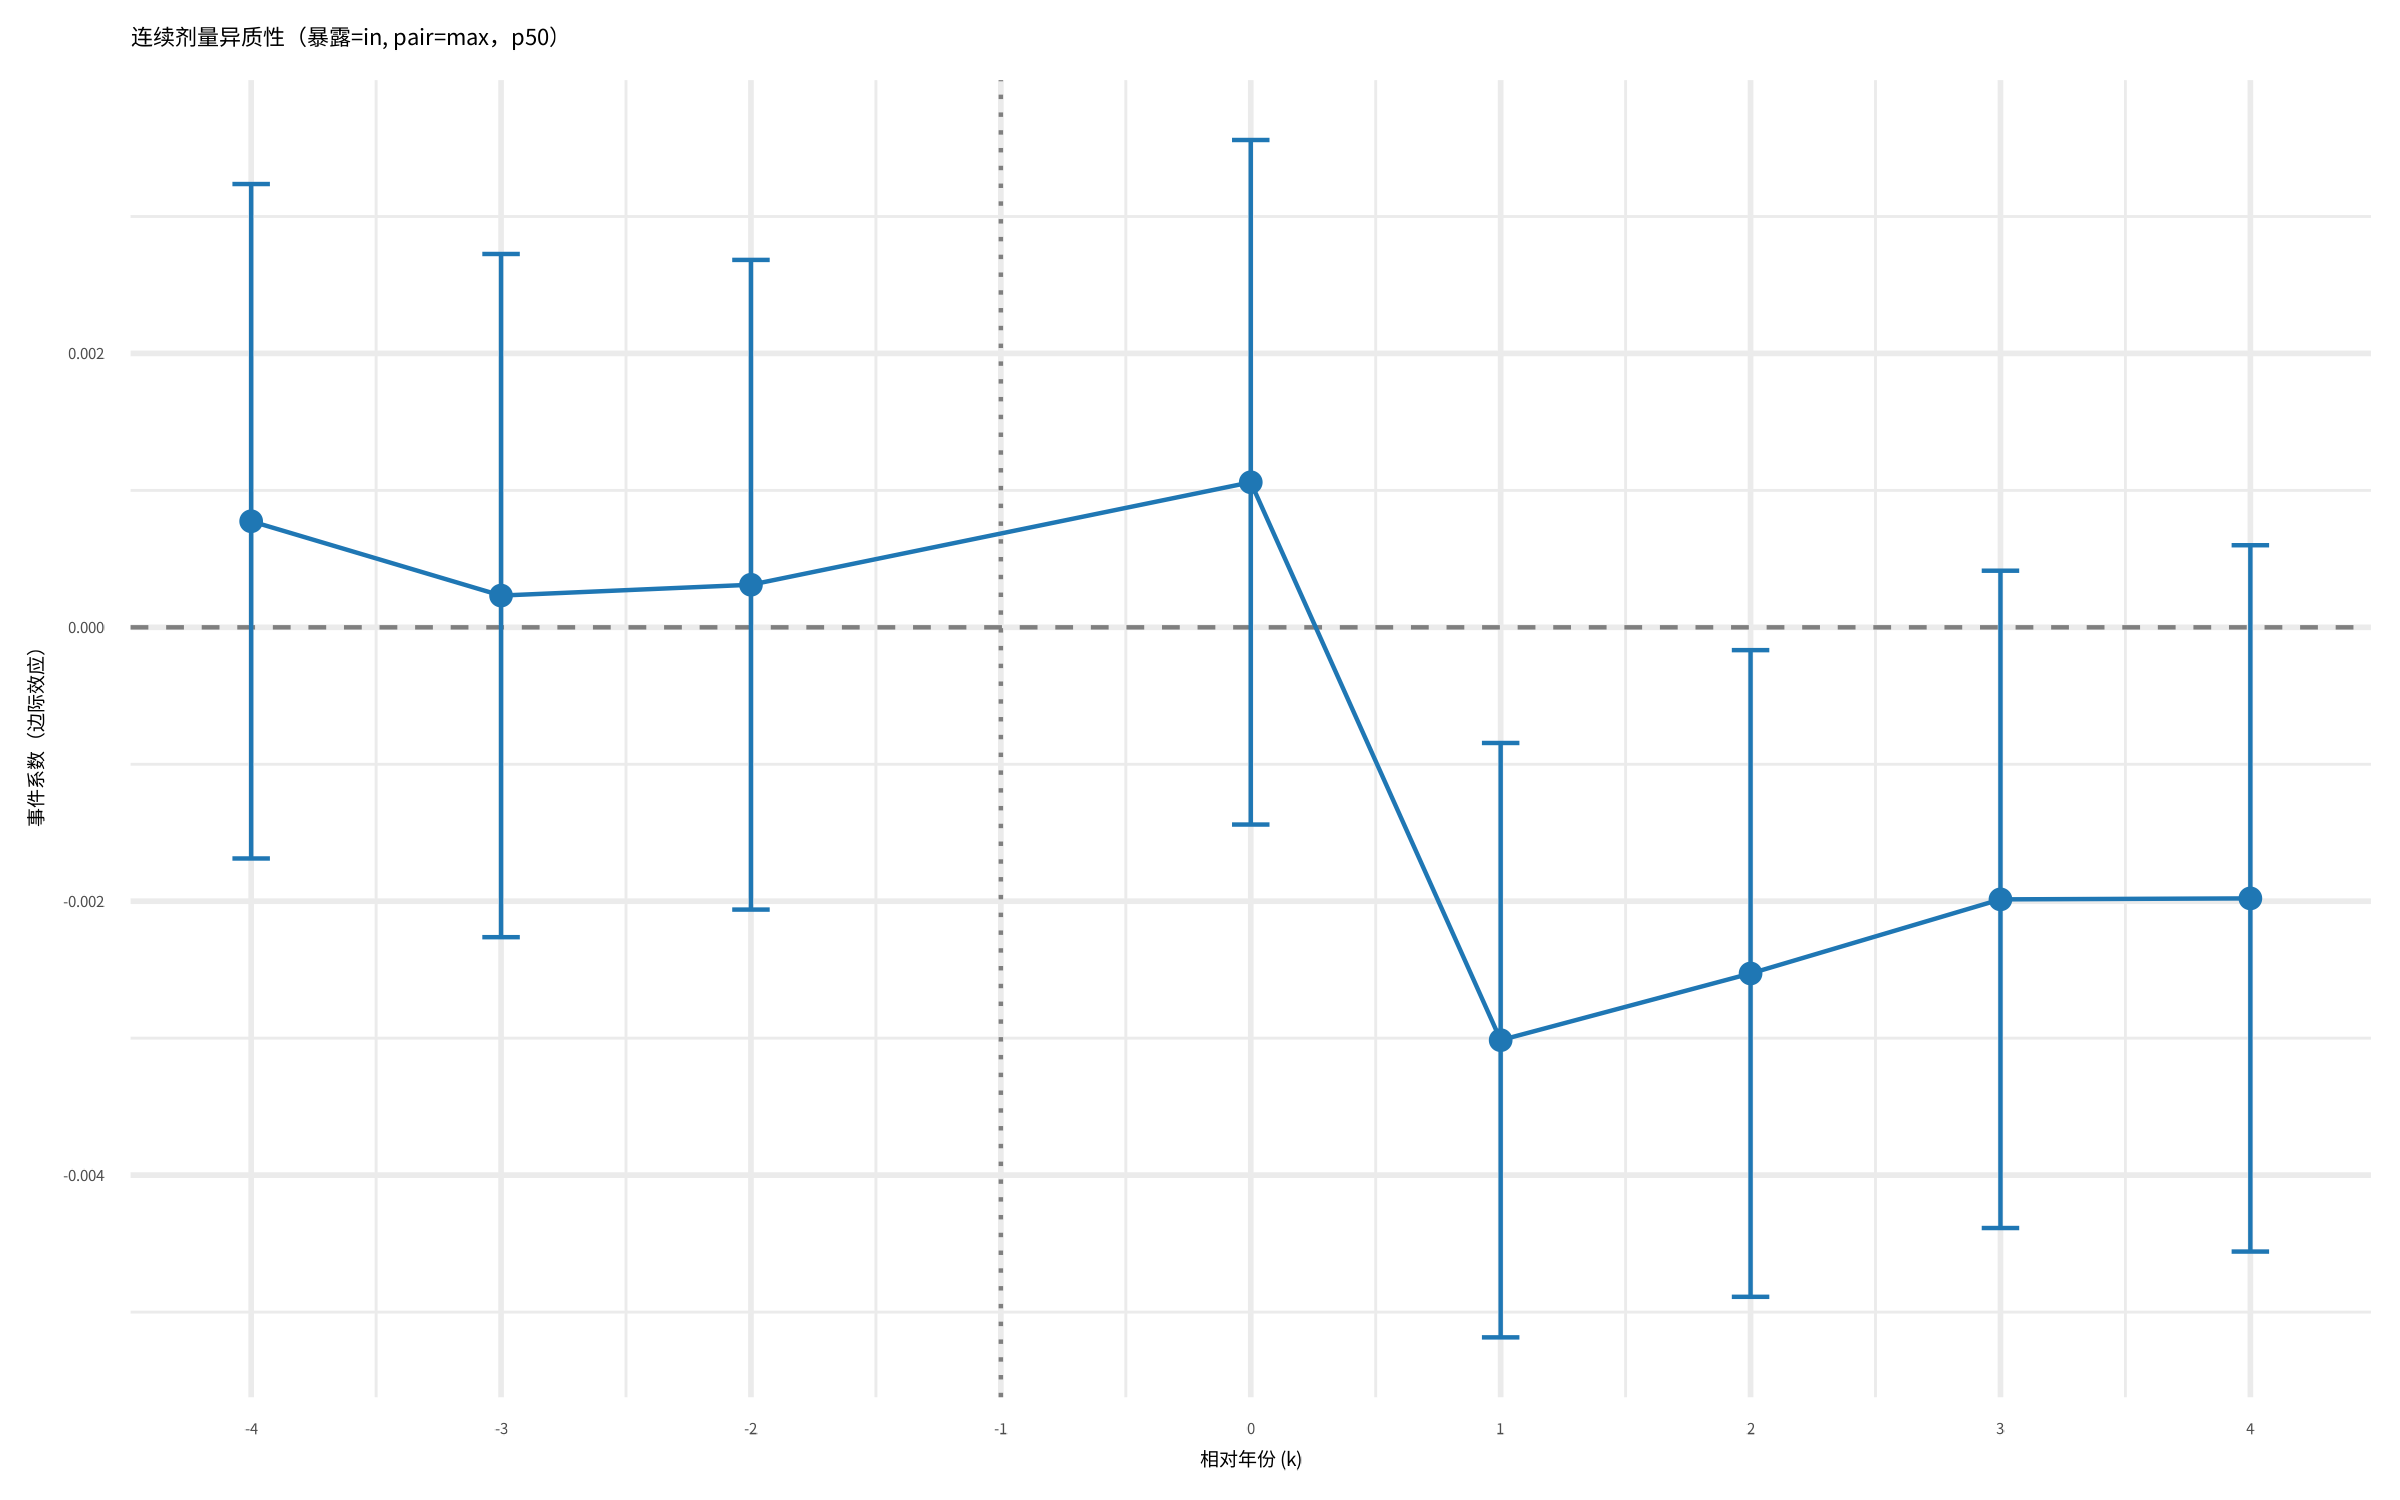
\includegraphics[width=0.85\linewidth]{figures/PT_exposure_cont_in_max_cont_p50.png}
  \caption{连续剂量(\(in\), pair=\(\max\)):中位暴露(p50)事件研究系数(95\%CI)。基准年 -1=2013。}
  \label{fig:hetero_expo_cont_in_p50}
\end{figure}

\begin{figure}[!htbp]
  \centering
  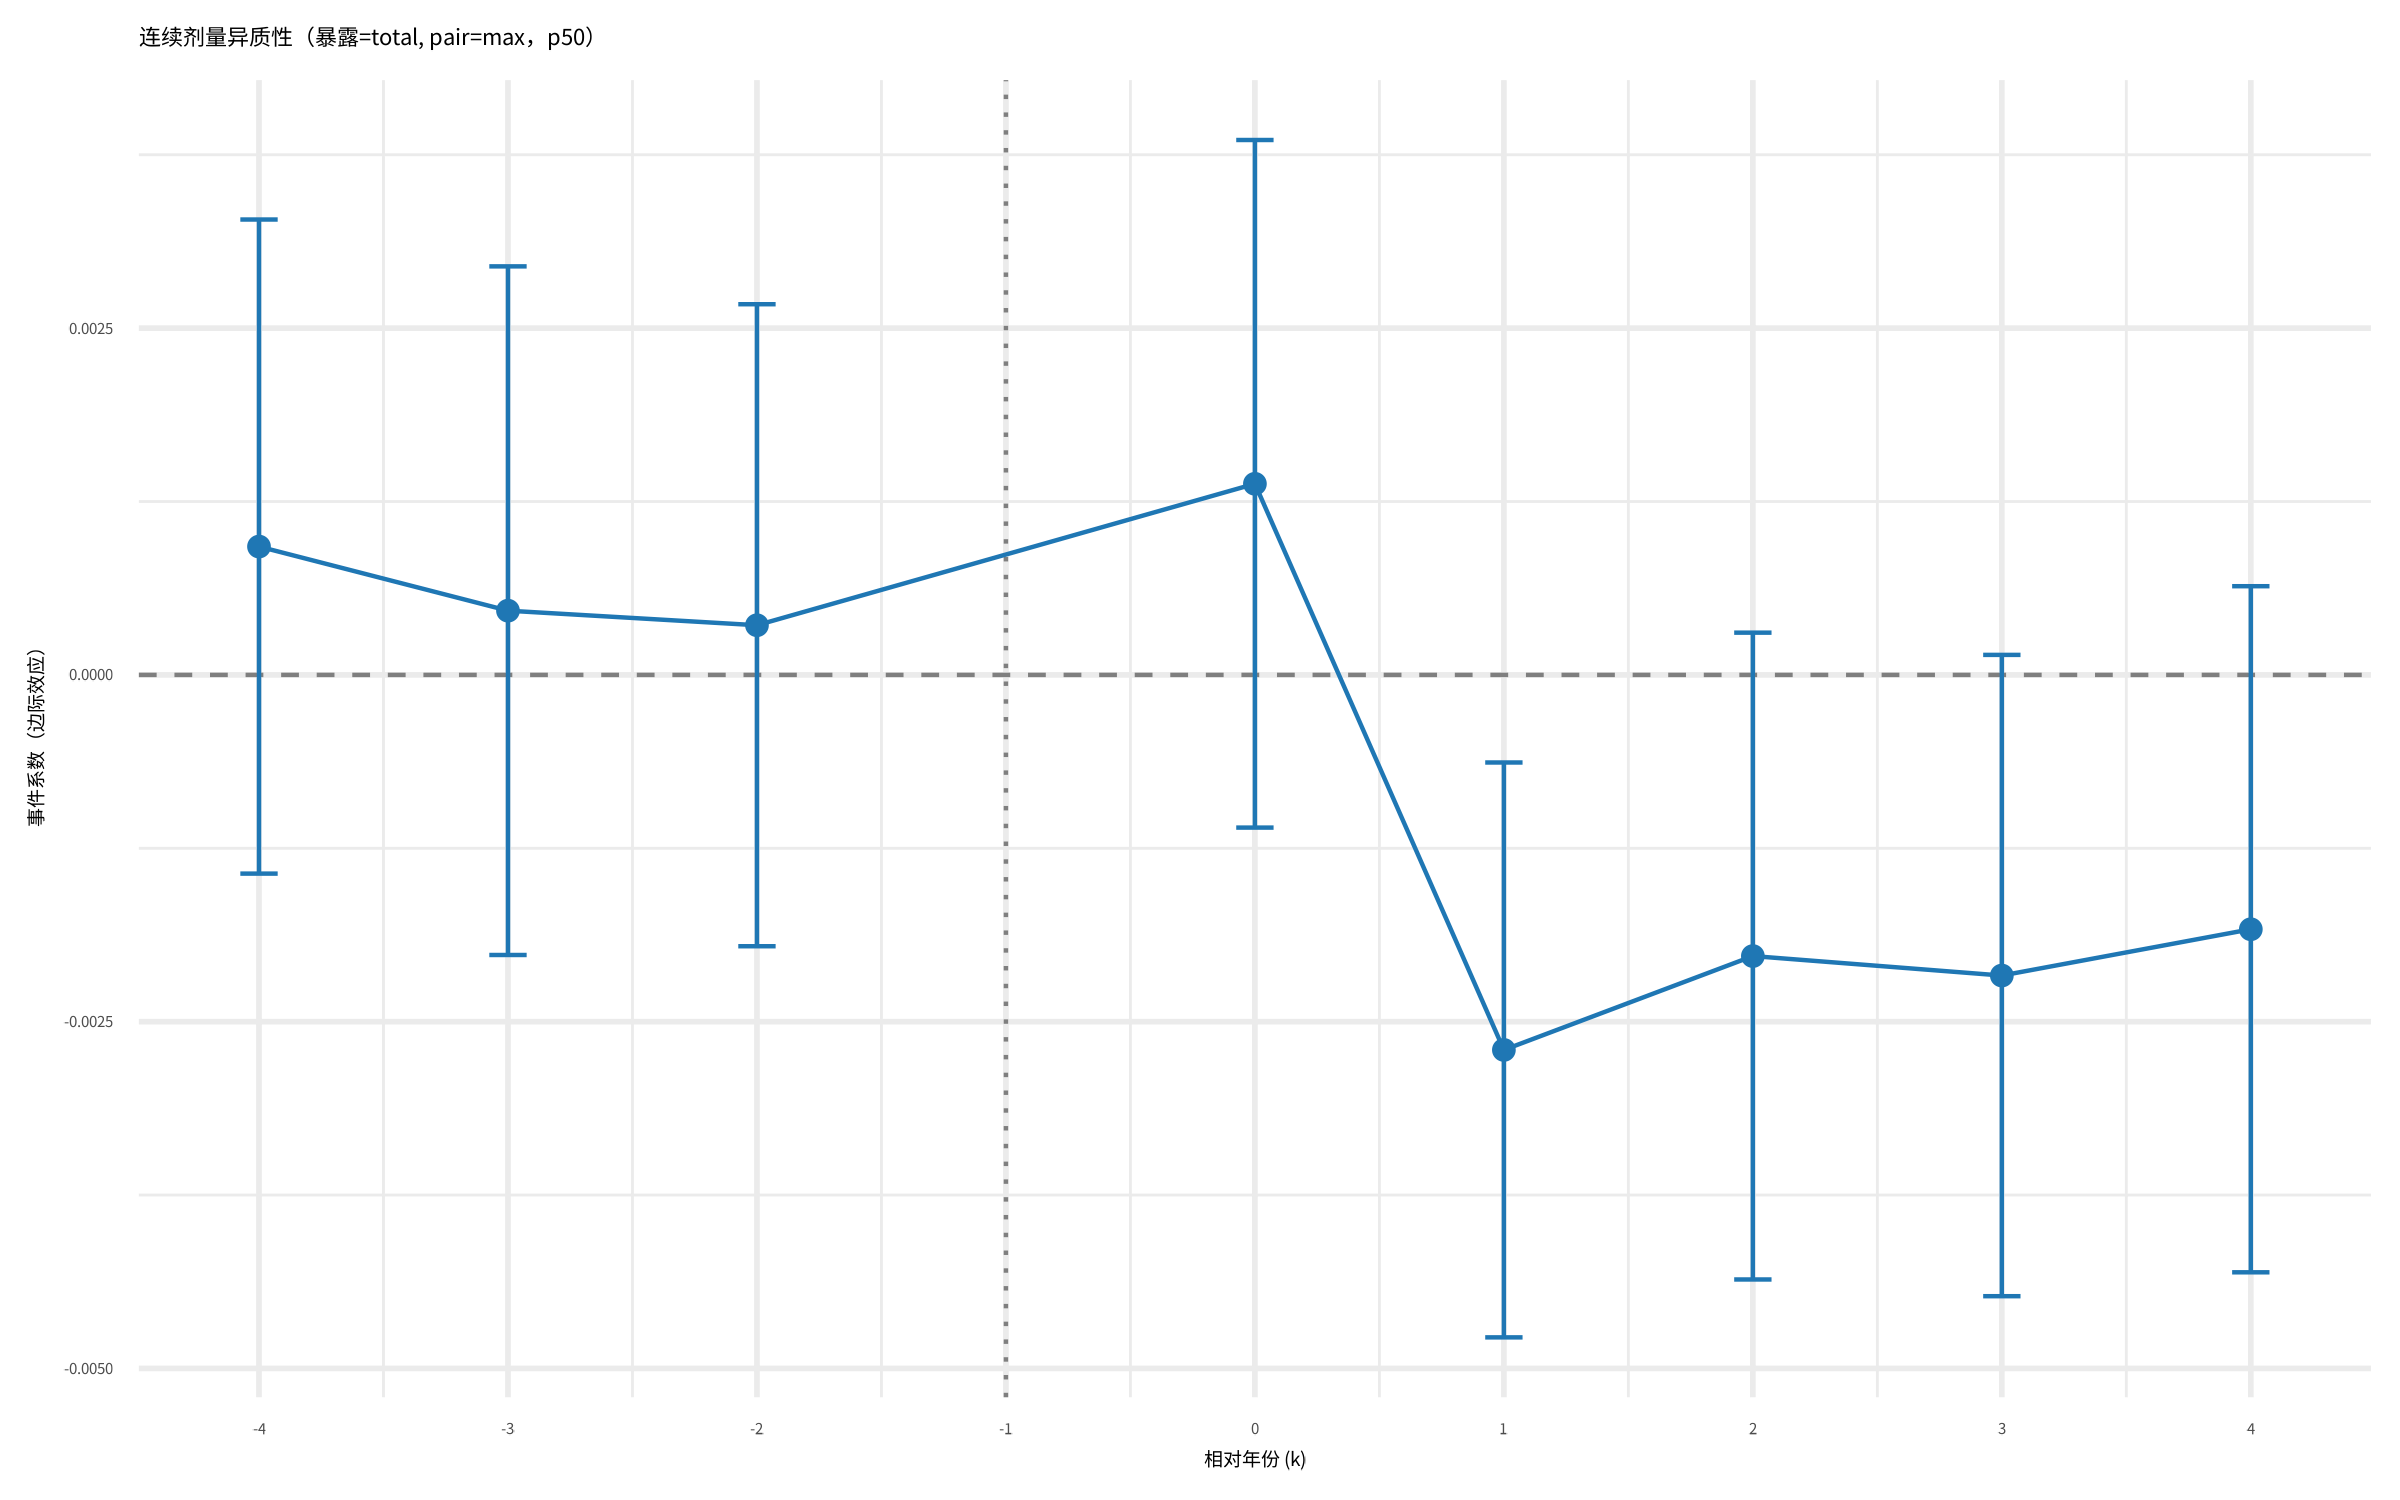
\includegraphics[width=0.85\linewidth]{figures/PT_exposure_cont_total_max_cont_p50.png}
  \caption{连续剂量(\(total\), pair=\(\max\)):中位暴露(p50)事件研究系数(95\%CI)。基准年 -1=2013。}
  \label{fig:hetero_expo_cont_total_p50}
\end{figure}

\paragraph{说明}
- 本节正文仅报告代表性水平(p50),以便聚焦“典型剂量”的因果图景;低/高分位(p25/p75)的完整曲线与事前/事后联合检验移至附录,透明呈现剂量—响应的稳健性(参见 \citet{sun2021event})。
- 交互项的整体方向与显著性为正文结论提供不依赖分位点的佐证:剂量越高,政策后抑制越强。

